% !TEX root = ../Abschlussbericht_Schimmeliger_Keller.tex
%%
%%  Hochschule für Technik und Wirtschaft Berlin --  Projektabschlussbericht
%%
%% Kapitel 4 - Praktische Umsetzung
%%
%%

\chapter{Praktische Umsetzung} \label{Praktische Umsetzung}
\section{Verwendete Hardware} \label{Hardware}
\subsection{LoPy4-Development-Board} \label{LoPy4}



\subsection{DHT Sensormodul} \label{DHT}

Bei dem verwendeten Sensor handelt es sich um einen sog. DHT Sensor. Diesen gibt es in zwei verschiedenen Ausführungen, DHT11 und DHT22, wobei sich diese im auswertbaren Messbereich, der Messgenauigkeit und im Preis unterscheiden.

\begin{adjustwidth}{-1in}{-1in}% adjust the L and R margins by -1 inch
	\begin{center}
	
	        \begin{tabular}{ccc}
			\toprule
			 & \textbf{DHT11} & \textbf{DHT22}\\

			\midrule
			Betriebsspannung & \multicolumn{2}{c}{3 \dots 5 V DC}\\
			Stromverbrauch & \multicolumn{2}{c}{max. 2,5 mA während der Konvertierung}\\
			Temperaturbereich & -20\dots 60 °C & -40\dots 80 °C  \\
			Temperatur Genauigkeit & ± 2,0 °C & ± 0,5 °C\\
			Feuchtigkeit Messbereich & 20\%\dots90\% RH & 0\%\dots99,9\% RH\\
			Feuchtigkeit Genauigkeit & ± 5,0\% RH & ± 2\dots5\%\\
			Abtastrate & 1 Hz & 0,5 Hz \\

			\midrule
			Preis (bei reichelt elektronik) & 1,80 € & 6,80 €\\

			\bottomrule
	
	        \end{tabular}
		\label{}
		\captionof{table}{Vergleich DHT11 zu DHT22} \label{tab:vergleichDHT} 
	\end{center}
\end{adjustwidth}

Anzumerken ist noch, dass der DHT22 Sensorungefähr das doppelte Volumen des DHT11 Sensors hat. Interessant ist auch, dass der DHT11 Sensor ungefähr doppelt so häufig angesprochen werden kann, was vermutlich auf seiner weniger komplexen Schaltung beruht.\\
Für die meisten Anwendungsfälle würde wahrscheinlich ein DHT11 Sensor (oder mehrere parallel geschaltete DHT11 Sensoren) ausreichen, um ein weitgehend zuverlässiges Ergebnis zu erhalten.

\subsubsection{Kommunikation mit dem DHT Sensor\cite{dht}} 

Die Kommunikation mit dem DHT Sensor erfolgt über eine einzelne Leitung, was zum einen die Kosten reduziert, zum anderen aber auch die Reichweite der störungfreien Übertragung erhöht. Um den Sensor anzusprechen und die Daten anschließend auszulesen, muss der Datenstrom kodiert werden. Dies geschieht über ein Protokoll, welches die Kommunikation in drei Schritte aufteilt:
\begin{itemize} 
	\item Request (die Anfrage)
	\item Repsonse (die Antwort des Sensors)
	\item Data (die vom Sensor übertragenen Daten)
\end{itemize}


\begin{center}
	\begin{figure}[h]
	 
	 \noindent\makebox[\textwidth]{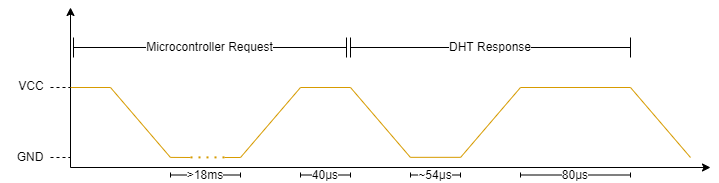
\includegraphics[width=1.1\textwidth]{pictures/dht_kommunikation1}}
	 \caption[DHT Kommunikation]{DHT Kommunikation}
	 \label{fig:dhtkommunikation}
	\end{figure}
\end{center}


Um den DHT Sensor dazu zu bringen, Messewerte zu senden, zieht der Microcontroller den Datenbus für mindestens 18ms auf Masse, um ihn anschließend für 40µs wieder auf Versorgungsspannungsniveau zu ziehen. Dadurch versteht der DHT Sensor, dass er beginnen soll Messwerte zu sammeln.\\
Der DHT Sensor antwortet zunächst mit einer Sequenz, bestehend aus einem ca. 54µs langen LOW und anschließend 80µs HIGH. 

\newpage

Nachfolgend sendet der DHT Sensor fünf Datenpakete, bestehend aus jeweils 8 Bit, welche die einzelnen Sensor Messwerte mit einer Prüfsumme darstellen. Insgesammt sendet der DHT Sensor somit 40 Bit.

\begin{center}
	\begin{figure}[h]
	 
	 \noindent\makebox[\textwidth]{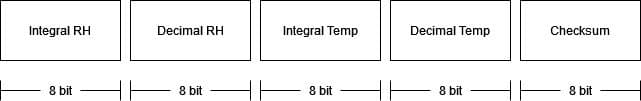
\includegraphics[width=0.9\textwidth]{pictures/dht11_dataframe}}
	 \caption[DHT Paketstruktur]{DHT Paketstruktur}
	 \label{fig:dhtpaketstruktur}
	\end{figure}
\end{center}

Die einzelnen Sensor Messwerte sind noch in Integral Anteil und Dezimal Anteil unterteilt, wobei die einzelnen Bits sich durch die dauer des HIGH Signals nach einem 54µs langem LOW Singal unterscheiden.

\begin{center}
	\begin{figure}[h]
	 
	 \noindent\makebox[\textwidth]{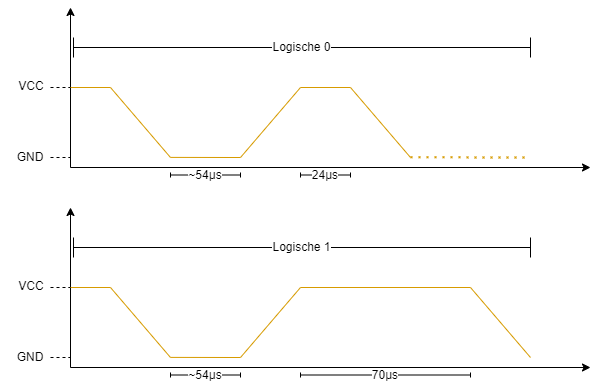
\includegraphics[width=0.9\textwidth]{pictures/dht_kommunikation2}}
	 \caption[DHT Bit Identifikation]{DHT Bit Identifikation}
	 \label{fig:dhtbits}
	\end{figure}
\end{center}

Abschließend sendet der DHT Sensor ein ca. 54µs langes LOW Signal, wonach der Bus wieder auf Versorgungsspannungsniveau gezogen wird und der Sensor in den Idle Mode geht.



\newpage

\subsection{Restliche Hardware} \label{Restliche Hardware}


\begin{itemize} 
	\item \textbf{Antenne:}  Bei der verwendeten Antenne handelt es sich um eine Multiband Antenne, welche für mehrere Freuquenzbänder (unter anderem das LoRa Freuquenzband) genutz werden kann.
	\item \textbf{USB Kabel:} Wir verwenden ein Daten-USB Kabel welches besonders geschirmt ist und eine maximal Länge von ca. 10cm aufweist. Wir hatten teilweise Probleme mit anderen USB Kabeln.
\end{itemize}



\section{Beschreibung der Software} \label{Software}

Für unser Projekt haben wir drei verschiedene, miteinander interagierende Software Komponenten realisiert, welche über eine Schnittstelle (Interface) miteinander kommunizieren. 
Der Vorteil einer solchen Architektur ist, dass die einzelnen Komponenten sich unter umständen wiederverwenden lassen und sich im Idealfall so eine Software modular aufbauen lässt.
Da wir als Programmiersprache ausschließlich Python bzw. Micropython verwendet haben, könnte man argumentieren, dass unsere Software automatisch Modular ist, da sich in der Theorie alle programmierten Komponenten in Python wiederverwenden lassen.
Dies ist aber sehr verallgemeinert gesprochen, da gerade die Programmierung der Mikrocontroller definitiv auch Individualsoftware benötigt, welche sich aber immerhin nicht nur auf einer einzelnen Mikrocontrollerfamilie ausführen funktionieren würde.
Anzumerken ist noch, dass für unsere finale Version des Projektes vermutlich nur eine einzelne Softwarekomponente notwendig wäre.\\
Für die Programmierung der Mikrocontroller verwenden wir die Programmiersprache Micropython, welche eine schlanke und schnelle Implementation der Programmiersprache Python ist, welche für Mikrocontroller optimiert wurde.

\newpage


\subsection{1. Komponente: Sensoransteuerung und der Versand der Daten mittels LoRa(WAN)} \label{Sender}


\begin{center}
	\begin{figure}[h]
	 
	 \noindent\makebox[\textwidth]{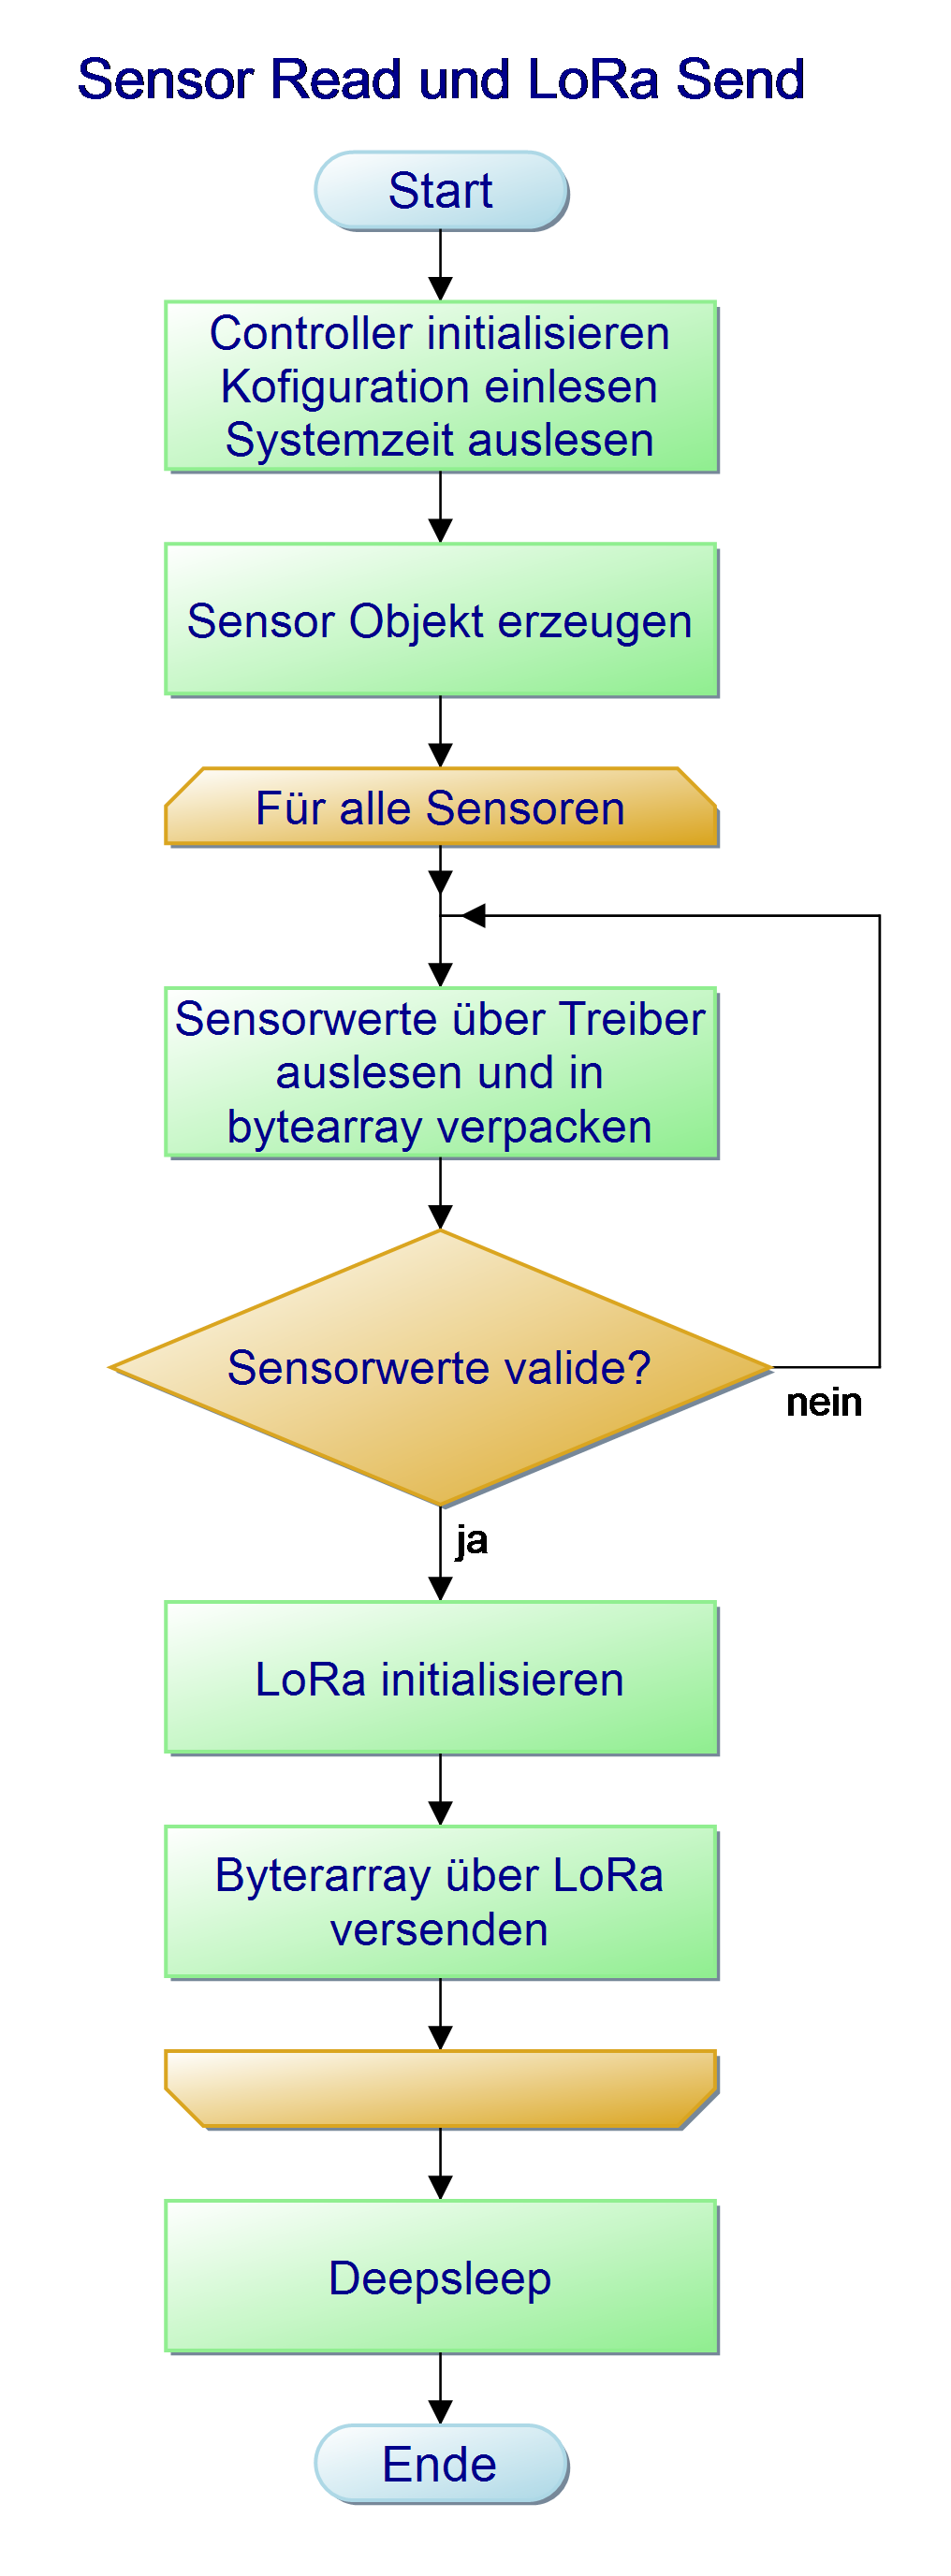
\includegraphics[width=0.35\textwidth]{pictures/sens_read_lora_send}}
	 \caption[PAP komponente 1]{Programm Ablauf: Komponente 1}
	 \label{fig:lorasendsensorread}
	\end{figure}
\end{center}

Zunächst wird der Microcontroller initialisiert, wobei er standartmäßig mit allen Modulen (WiFi, LoRa, etc.) im aktivierten Zustand startet. Dieser Umstand beruht darauf, dass wir die PyCom Plattform nutzen, welche wenig vorab Konfiguration ermöglicht.

\newpage

\subsection{2. Komponente: Emfangen der Daten und Versand ins Internet} \label{Empfänger}

\begin{center}
	\begin{figure}[h]
	 
	 \noindent\makebox[\textwidth]{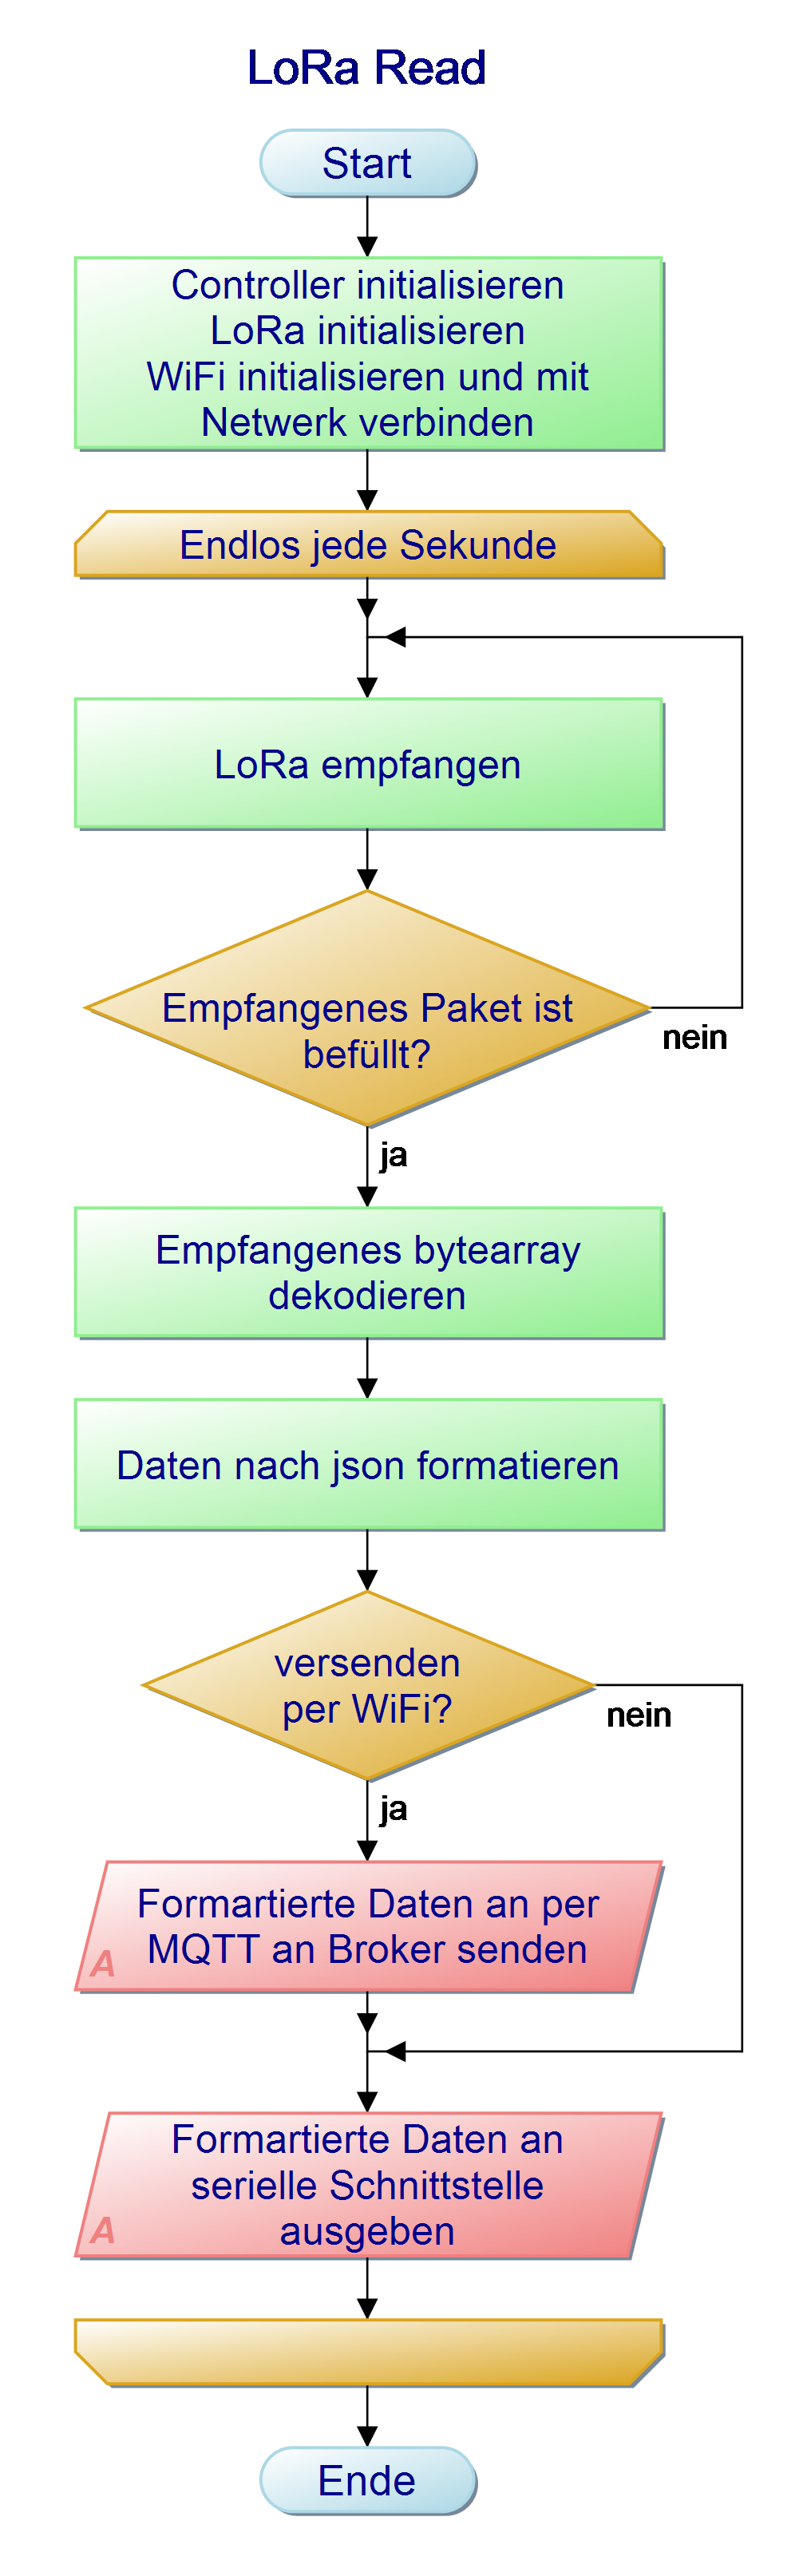
\includegraphics[width=0.3\textwidth]{pictures/LoRaRead}}
	 \caption[PAP komponente 2]{Programm Ablauf: Komponente 2}
	 \label{fig:lorareadwifisend}
	\end{figure}
\end{center}

abc

\newpage

\subsection{3. Komponente: Manuelles abrufen und versenden der veröffentlichten Daten} \label{PubSub}

\begin{center}
	\begin{figure}[h]
	 
	 \noindent\makebox[\textwidth]{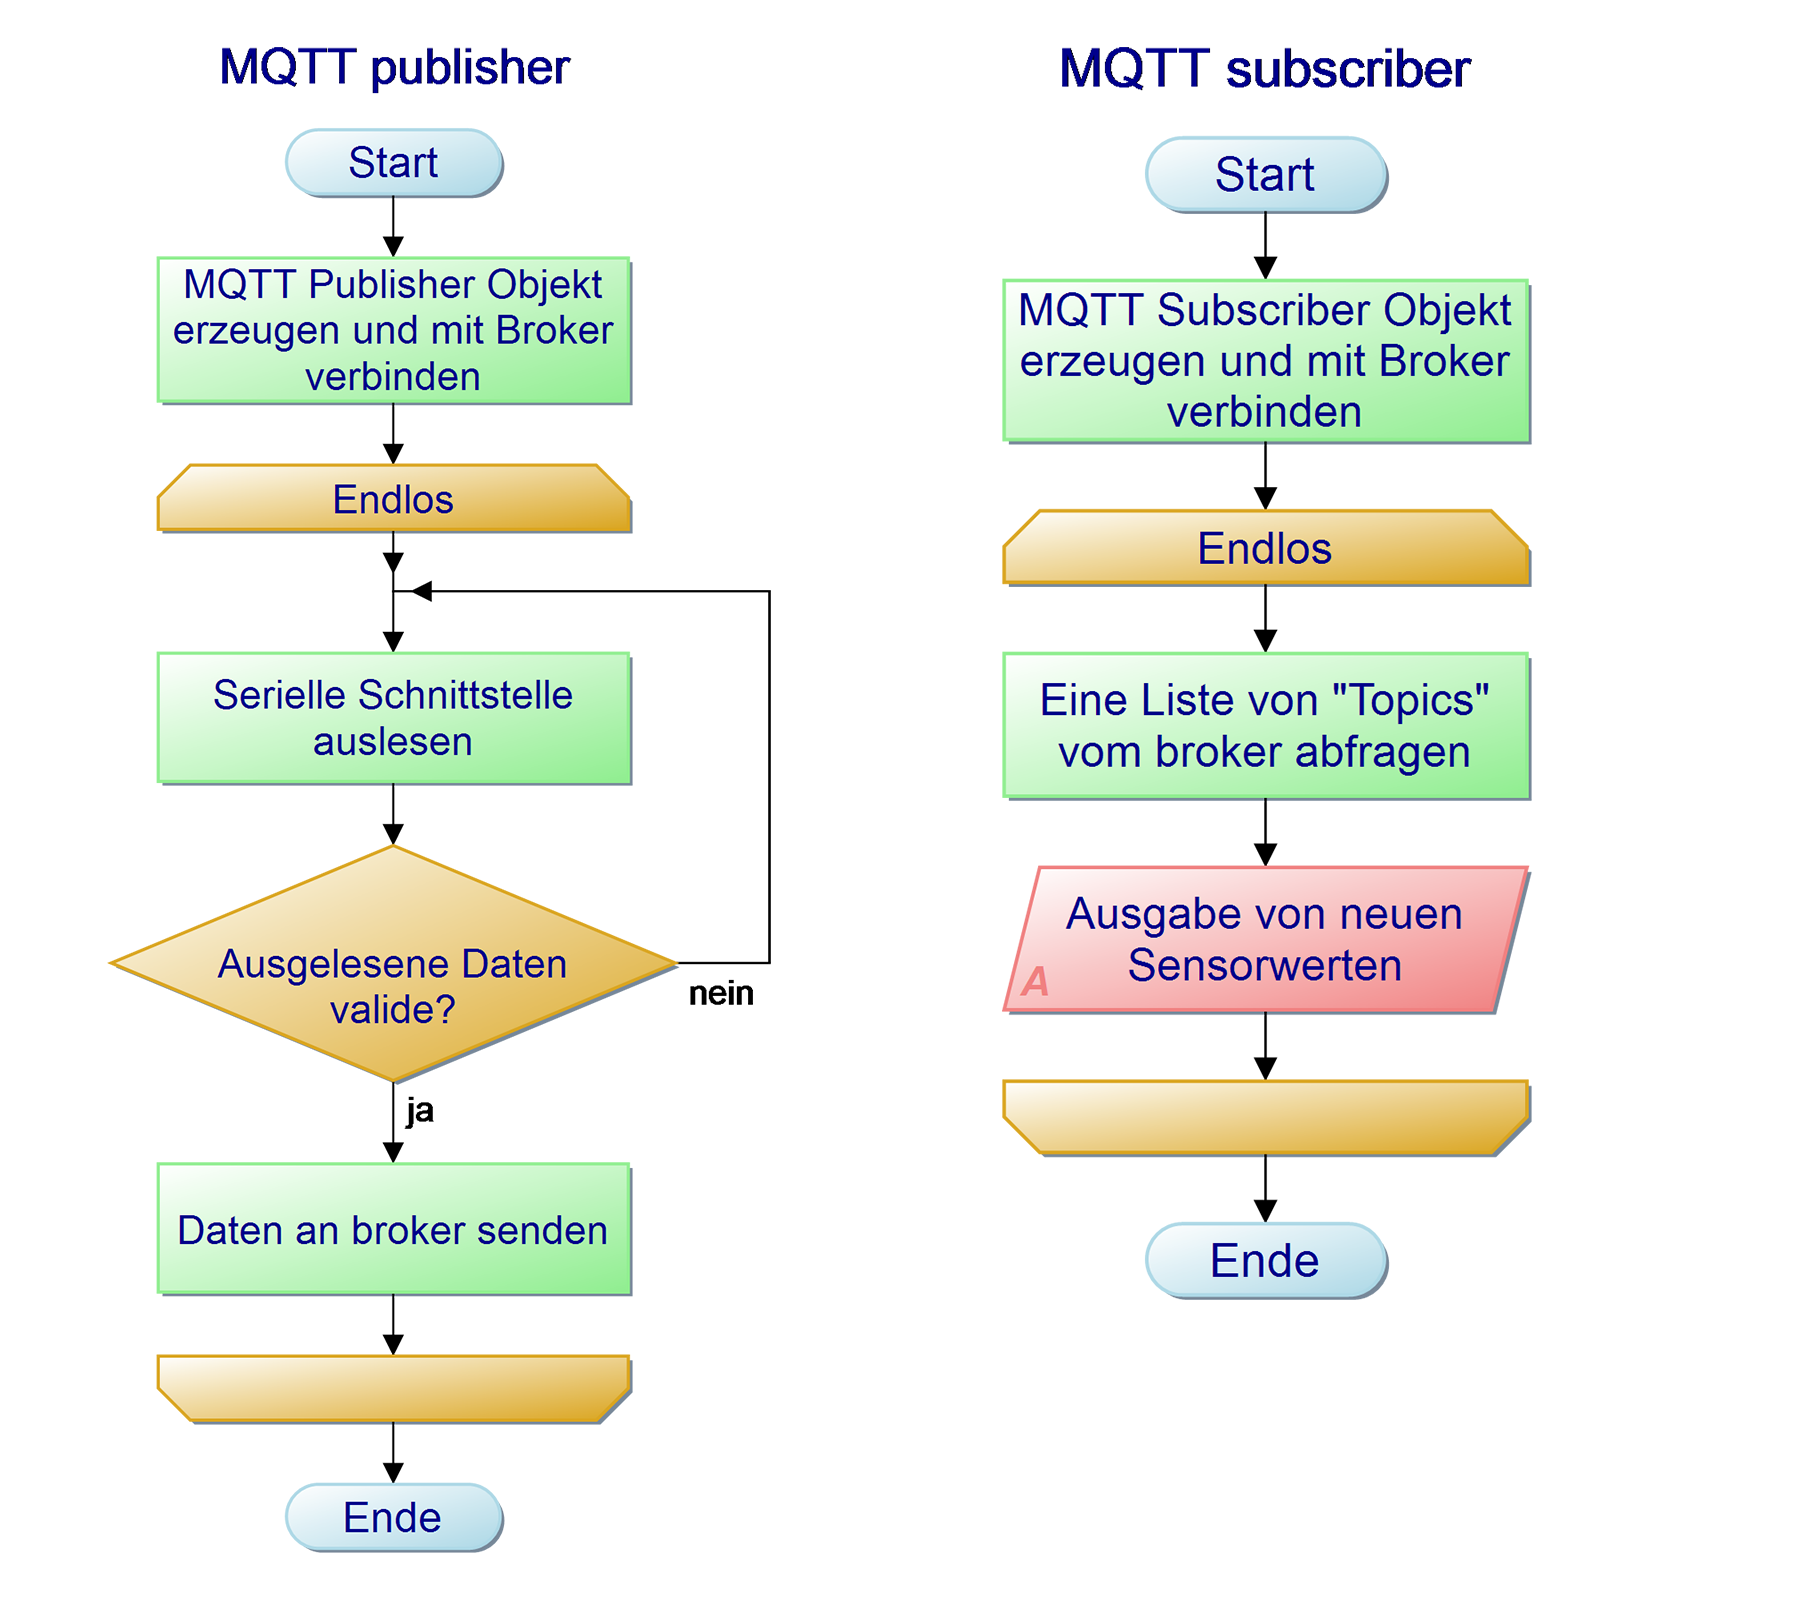
\includegraphics[width=0.9\textwidth]{pictures/MQTTpubsub}}
	 \caption[PAP komponente 3]{Programm Ablauf: Komponente 3}
	 \label{fig:MQTTpubsub}
	\end{figure}
\end{center}

abc

\newpage

\section{Visualisierung der Sensordaten} \label{Dashboard und Visualisierung}

abc

\newpage


\section{Berechnung der Laufzeit im Batteriebetrieb} \label{Simulation}

\begin{center}
	\begin{figure}[h]
	 
	 \noindent\makebox[\textwidth]{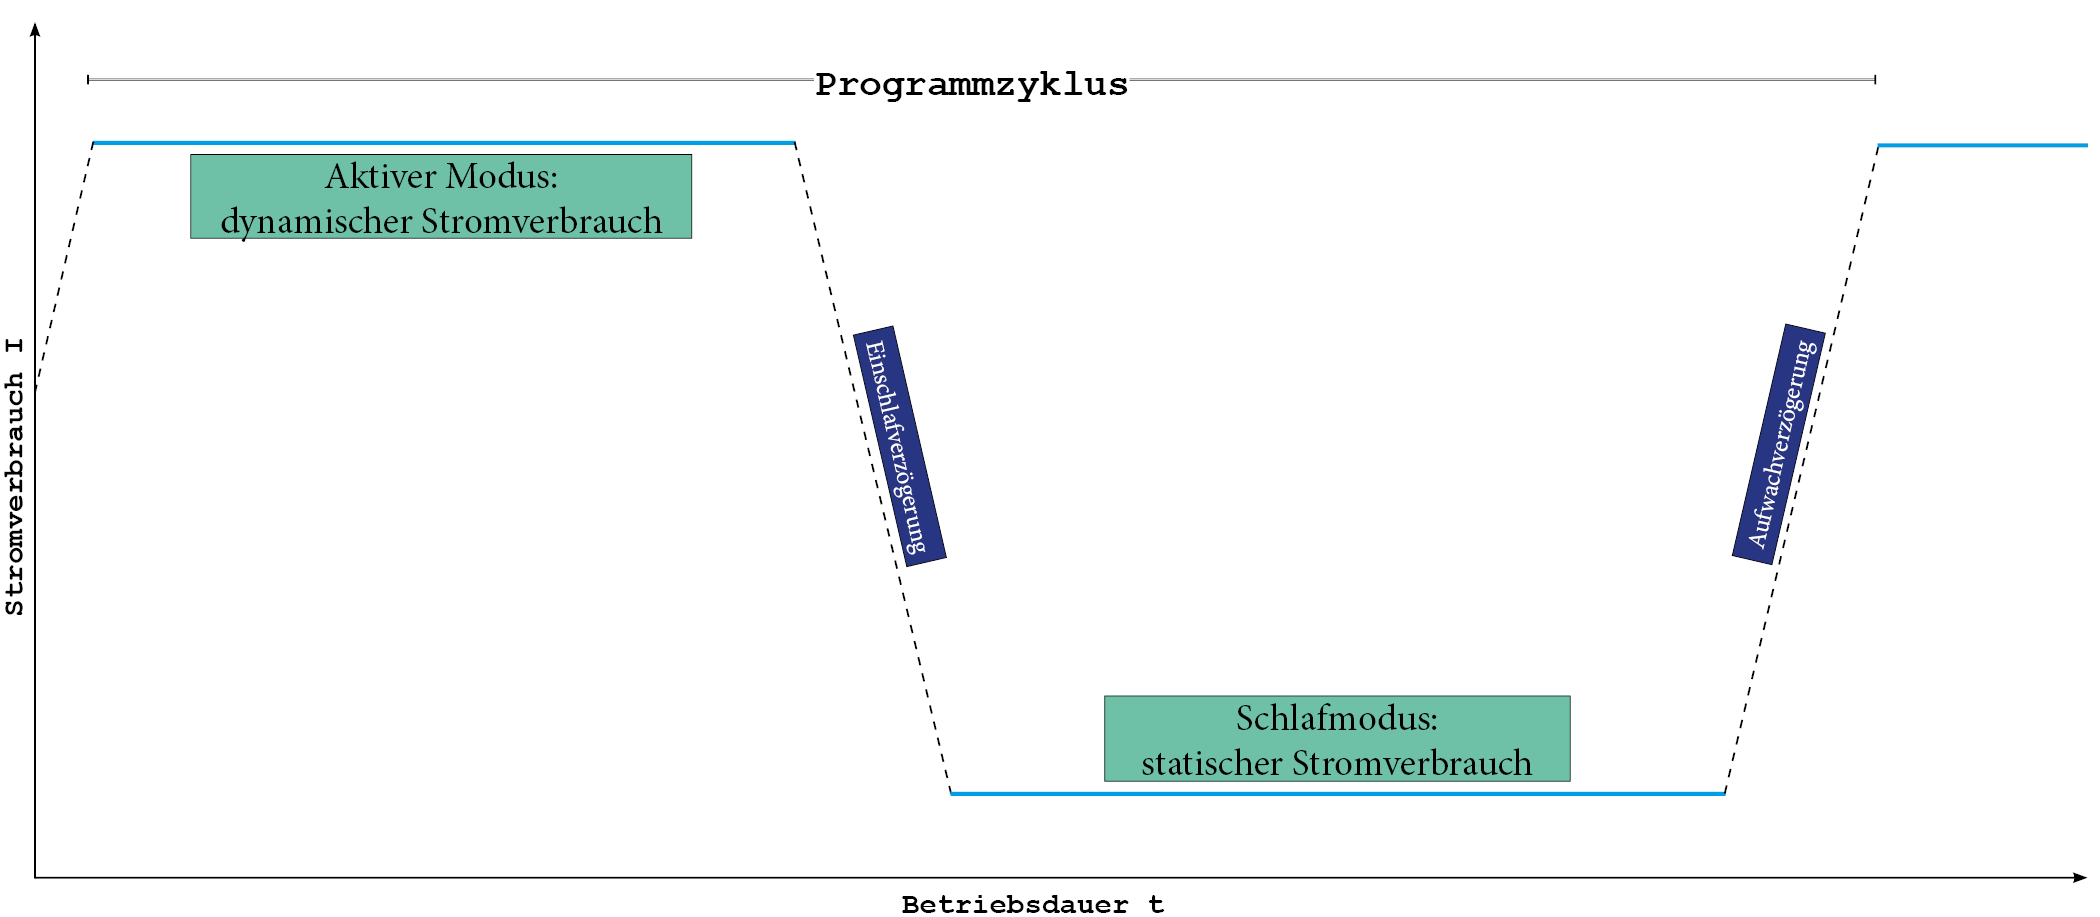
\includegraphics[width=1.1\textwidth]{pictures/programmzyklus}}
	 \caption[Stromverbrauch während eines Programmzyklus]{Stromverbrauch während eines Programmzyklus}
	 \label{fig:stromzyklus}
	\end{figure}
\end{center}

abc

\newpage
